\subsection{Численные примеры неустойчивых решений уравнения теплопроводности}
\vspace{1em}

\newtheorem{exmp}{Пример}

\begin{exmp}
\end{exmp}

В качестве начальных условий выберем $u_0 = \sin(\pi x)$. Рис. 1. иллюстрирует 
неустойчивость нулевого решения при $\alpha = \pi^2 + 0.1$.

\begin{figure}[H]
    \centering
        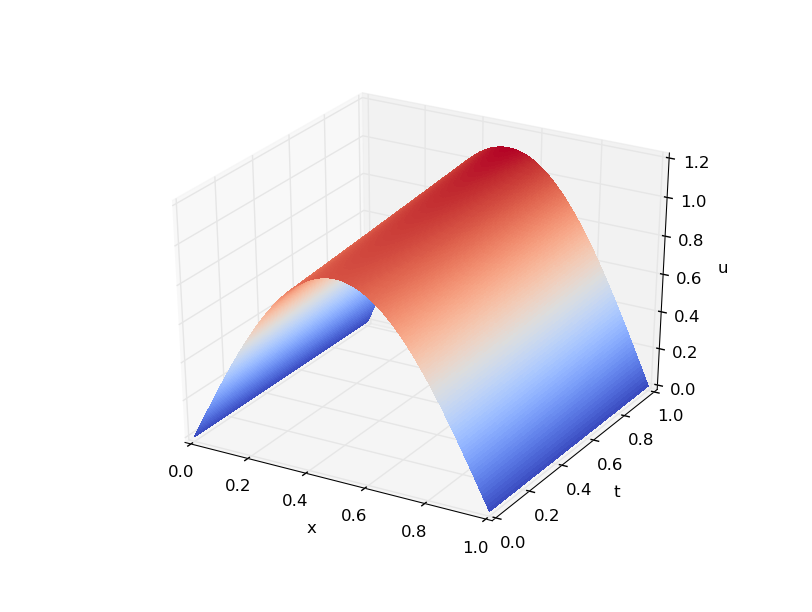
\includegraphics[width=3.5in]{par_ex_pi01}
        \caption{}
        \label{fig:test1}
\end{figure}

\begin{exmp}
\end{exmp}

На рис. 2 приведен график решения задачи \eqref{dif_form} - \eqref{d_control}
при $\alpha = \pi^2 + 3$ и $u_0(x) = x(1 - x)$, который демонстрирует 
экспоненциальный рост решения при увеличении $t$.

\begin{figure}[H]
    \centering
        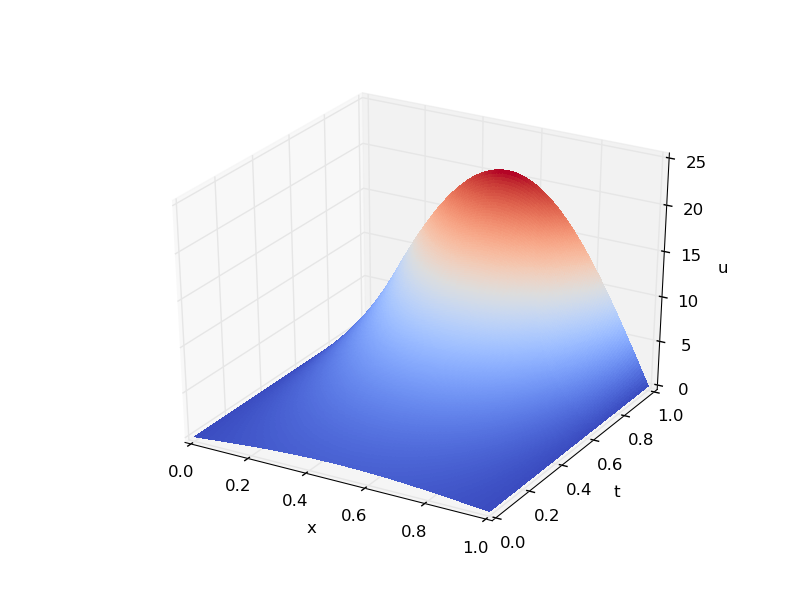
\includegraphics[width=3.5in]{par_ex_pi3}
        \caption{}
        \label{fig:test1}
\end{figure}

